%%%%%%%%%%%%%%%%%%%%%%%%%%%%%%%%%%%%%%%%%%%%%%%%%%%%%%%%%%%%%%%%%%%%%%%%%%%%
%  第25回 例題21・22（原本 20161215144626.pdf の PDFページ1・3＝原本 p5 / p9 より）
%  原本は「問題枠 →(指針)空欄→【KEY】」で解答が載っていないため，
%  【指針】と【解答】は本文の説明・練習問題の解答の解き方に合わせて書き起こした．
%  （例題22 の指針だけは原本にも記述があるので，それを含めてある）
%  ※ このファイルは記録用。実体は physics_ch25.tex に流し込み済み。
%%%%%%%%%%%%%%%%%%%%%%%%%%%%%%%%%%%%%%%%%%%%%%%%%%%%%%%%%%%%%%%%%%%%%%%%%%%%

%%%%%%%%%%%%%%%%%%%%  例題21（25.1 のまとめ枠の直後）  %%%%%%%%%%%%%%%%%%%%
\begin{reidaiunit}
\begin{reidai}{ヤングの実験}
\begin{zuright}{78mm}
\hspace{1zw}波長$\lambda\U{m}$の光を出す単色光源を用意し，単スリット$\mathrm{A}$，複スリット$\mathrm{B}$，スクリーン$\mathrm{C}$をこの順に平行に設置する．スクリーン$\mathrm{C}$上の点$\mathrm{P}$では，光源から出て$\mathrm{S_0\to S_1\to P}$の経路をたどる光と，$\mathrm{S_0\to S_2\to P}$の経路をたどる光が干渉する．

\hspace{1zw}複スリットのスリット間隔$\overline{\mathrm{S_1S_2}}$を$d\U{m}$，$\mathrm{BC}$間の距離を$l\U{m}$，$\overline{\mathrm{OP}}=x\U{m}$として以下の問に答えよ．ただし，$\mathrm{S_1}$と$\mathrm{S_2}$はともに$\mathrm{S_0}$から等距離にあり，$d\ll l$, $x\ll l$であるとして良い．
\zusep
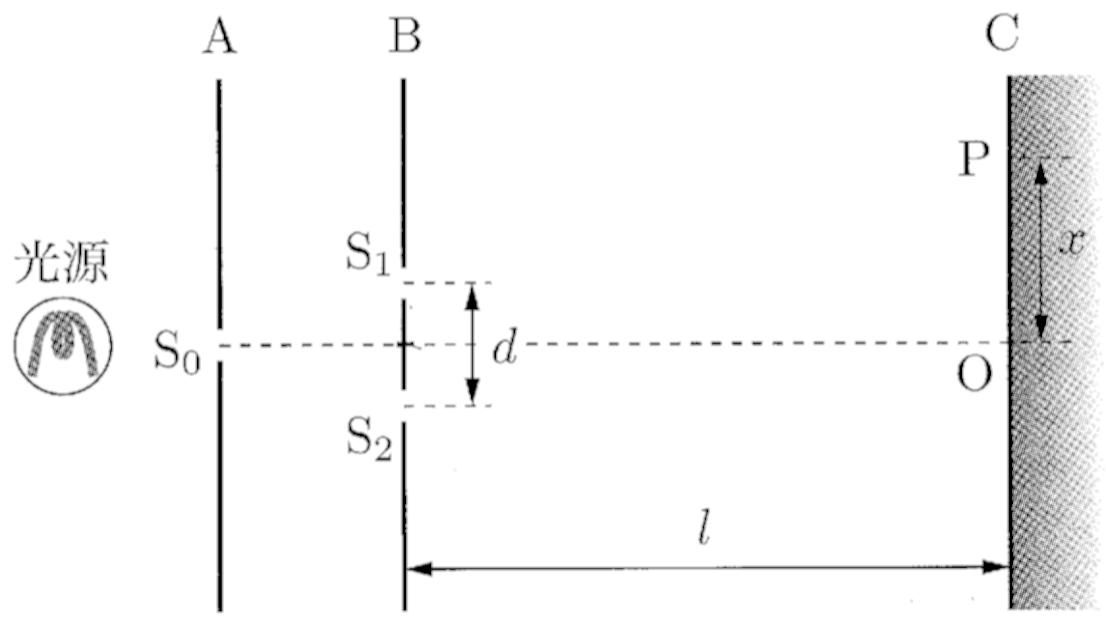
\includegraphics[keepaspectratio,width=78mm]{fig/ch25_ex21_young.png}
\end{zuright}
\begin{komon}
\ko{1} $\overline{\mathrm{S_2P}}-\overline{\mathrm{S_1P}}$を近似して求めよ．
\ko{2} $\mathrm{P}$が強め合いとなっている条件を整数$m$を用いて表し，スクリーン$\mathrm{C}$上で明線となる位置を求めよ．
\ko{3} スクリーン$\mathrm{C}$上の明線間隔$\Delta x\U{m}$を求めよ．
\ko{4} (3)の結果より，複スリットのスリット間隔を広げると，明線間隔は広くなるか，狭くなるか答えよ．また，光の波長を長くした場合，明線間隔は広くなるか，狭くなるか答えよ．
\end{komon}
\end{reidai}

\begin{sisinE}
経路差は，スリットの中点$\mathrm{M}$から$\mathrm{P}$への振れ角$\theta$を用いて$d\sin\theta\fallingdotseq d\tan\theta$と求めるのが速い．厳密に三平方の定理から求めることもできる（練習問題［51］）．

$\mathrm{S_1}$, $\mathrm{S_2}$は同位相の波源であるから，反射による位相のずれを考える必要はなく，経路差が真空中の波長の整数倍かどうかだけで強め合い・弱め合いが決まる．

(4)は(3)で求めた$\Delta x=\dfrac{l\lambda}{d}$を見て，$d$・$\lambda$を変えたときに$\Delta x$が増えるか減るかを答えればよい．
\end{sisinE}

\Key{経路差$\Delta D$を求め，$\Delta D=m\lambda$のとき強め合い，$\Delta D=\left(m-\dfrac{1}{2}\right)\lambda$のとき弱め合い，から議論する．}

\begin{kaitou}
\begin{komon}
\ko{1} $\overline{\mathrm{S_1S_2}}$の中点を$\mathrm{M}$とし，$\angle\mathrm{PMO}=\theta$とおく．$d\ll l$であるから$\mathrm{S_1P}$, $\mathrm{MP}$, $\mathrm{S_2P}$は互いに平行とみなせる．$\mathrm{S_1}$から直線$\mathrm{S_2P}$に下ろした垂線の足を$\mathrm{H}$とすると$\overline{\mathrm{S_1P}}\fallingdotseq\overline{\mathrm{HP}}$であるから，
       \Ana{\overline{\mathrm{S_2P}}-\overline{\mathrm{S_1P}}\fallingdotseq\overline{\mathrm{S_2H}}=d\sin\theta}
       さらに$x\ll l$であるから$|\theta|\ll 1$であり，
       \Ana{\overline{\mathrm{S_2P}}-\overline{\mathrm{S_1P}}\fallingdotseq d\sin\theta\fallingdotseq d\tan\theta=d\frac{x}{l}\U{m}\Ans}
\ko{2} $\overline{\mathrm{S_0S_1}}=\overline{\mathrm{S_0S_2}}$であるから$\mathrm{S_1}$, $\mathrm{S_2}$は同位相の波源であり，経路差が波長の整数倍のときに$\mathrm{P}$点で強め合う．よって強め合いの条件は，$m$を整数として
       \Ana{d\frac{x}{l}=m\lambda\Ans}
       これを$x$について解いて，明線となる位置は
       \Ana{x=m\frac{l\lambda}{d}\U{m}\Ans}
\ko{3} (2)の$m$を1つずらして差し引くことにより，
       \Ana{\Delta x=(m+1)\frac{l\lambda}{d}-m\frac{l\lambda}{d}=\frac{l\lambda}{d}\U{m}\Ans}
\ko{4} $\Delta x=\dfrac{l\lambda}{d}$より，$\Delta x$は$d$に反比例し，$\lambda$に比例する．よって，スリット間隔$d$を広げると明線間隔は{\gtfamily 狭くなり}，波長$\lambda$を長くすると明線間隔は{\gtfamily 広くなる}．\hspace*{\fill}\Ans
\end{komon}
\end{kaitou}
\end{reidaiunit}

%%%%%%%%%%%%%%%%%%%%  例題22（25.4 のまとめ枠＋加筆の直後）  %%%%%%%%%%%%%%%%%%%%
% 例題22 のユニットは「問題枠＋図」で 90mm 近くあり，reidaiunit 既定の \bsNeed{30mm}
% では見出しだけがページ末に残ったり，枠が改ページで割れて Overfull \vbox が出る．
\bsNeed{95mm}
\begin{reidaiunit}
\begin{reidai}{回折格子}
\begin{zuright}{70mm}
\hspace{1zw}図のように，格子定数（溝の間隔）が$d\U{m}$の回折格子を水槽の底に置き，下方向から波長$\lambda\U{m}$の単色光を当てる．この際に出来る回折光が回折格子と垂直な方向となす角を反時計回りに$\theta\ \left(-\dfrac{\pi}{2}<\theta<\dfrac{\pi}{2}\right)$とする．空気の屈折率は1として以下の問いに答えよ．
\zusep
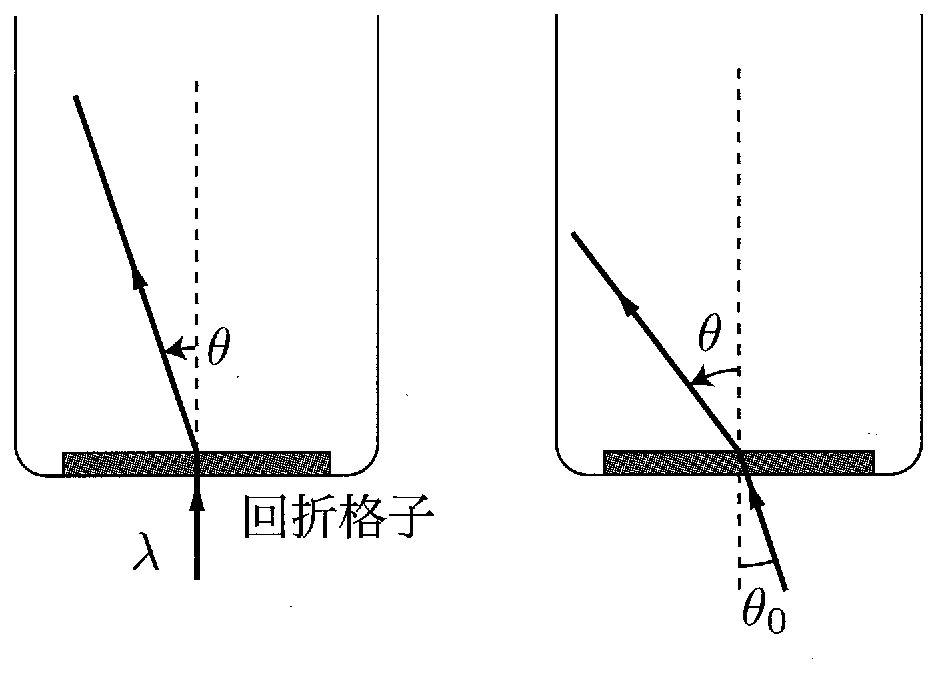
\includegraphics[keepaspectratio,width=70mm]{fig/ch25_ex22_grating.png}
\end{zuright}
\begin{komon}
\ko{1} 回折格子に対して垂直に入射した場合，$\sin\theta$の値を$d$, $\lambda$および整数$m$を用いて表せ．
\ko{2} 図のように，回折格子に垂直な方向と$\theta_0$の角度で入射した場合，$\sin\theta$の値を$d$, $\lambda$, $\theta_0$および整数$m$を用いて表せ．
\ko{3} 水槽に屈折率$n$の液体を入れ，回折格子に垂直な方向と$\theta_0$の角度で入射した場合，$\sin\theta$の値を$d$, $\lambda$, $\theta_0$, $n$および整数$m$を用いて表せ．
\end{komon}
\end{reidai}

\begin{sisinE}
垂直に入射した場合は，【KEY】の$d\sin\varphi=m\lambda$を考えればよい．斜めに入射した場合も，隣り合うスリットを通った光が強め合う条件を立てる．
% ここまでは原本の(指針)欄にある記述．以下はこちらで補った．

このとき，回折格子に{\gtfamily 入る前}にも隣り合う光の間には経路差が生じていることに注意する．$\theta$と$\theta_0$を図のように同じ向き（反時計回り）に測っていることに気をつけて，入射側と回折側の経路差を符号込みで足し合わせる．

(3)のように回折光が媒質中へ出ていく場合は，経路差ではなく{\gtfamily 光路差}（＝屈折率$\times$距離）を真空中の波長と比べる．
\end{sisinE}

\Key{角度$\varphi$方向での強め合い条件\quad$\Rightarrow$\quad$d\sin\varphi=m\lambda$}

\begin{kaitou}
\begin{komon}
\ko{1} 隣り合うスリットを通ってきた光の経路差は$d\sin\theta$であるから，強め合いの条件は
       \Ana{d\sin\theta=m\lambda}
       よって，
       \Ana{\sin\theta=\frac{m\lambda}{d}\Ans}
\ko{2} 隣り合う2つのスリットに入射するまでの間に，光はすでに$d\sin\theta_0$の経路差を持っている．回折した後にはさらに$d\sin\theta$の経路差がつくが，$\theta$と$\theta_0$を同じ向きに測っているため，この2つは互いに打ち消し合う向きになる．よって全経路の経路差は
       \Ana{\Delta D=d\sin\theta-d\sin\theta_0\U{m}}
       であるから，強め合いの条件は
       \Ana{d(\sin\theta-\sin\theta_0)=m\lambda}
       すなわち，
       \Ana{\sin\theta=\sin\theta_0+\frac{m\lambda}{d}\Ans}
       \begin{chuu}
       $m=0$とすると$\theta=\theta_0$，すなわち回折せずにまっすぐ進む光（0次の明線）になる．検算に使える．
       \end{chuu}
\ko{3} 回折格子より上は屈折率$n$の液体，下は空気（屈折率1）であるから，経路差ではなく光路差を真空中の波長$\lambda$と比べる．(2)の各経路差を光路長に直すと，光路差は
       \Ana{\Delta D=n\cdot d\sin\theta-1\cdot d\sin\theta_0\U{m}}
       であるから，強め合いの条件は
       \Ana{d(n\sin\theta-\sin\theta_0)=m\lambda}
       すなわち，
       \Ana{\sin\theta=\frac{1}{n}\left(\sin\theta_0+\frac{m\lambda}{d}\right)\Ans}
       \begin{chuu}
       $m=0$とすると$n\sin\theta=\sin\theta_0$となり，空気から液体への屈折の法則そのものになる．
       \end{chuu}
\end{komon}
\end{kaitou}
\end{reidaiunit}
